\documentclass[letterpaper,12pt]{article}
\usepackage[utf8]{inputenc}
\usepackage{geometry}
\usepackage{amsmath}
\usepackage{float}
\usepackage{graphicx}
\usepackage{subcaption}
\usepackage{amssymb}
\usepackage{adjustbox}
\usepackage{wrapfig} %%imagen envuelta por un texto
\usepackage{xcolor}
\usepackage{fancyhdr}

\title {\textbf{"Cálculo de una variable "}}
\author{Deniso Xocuis}
\date{5 de abril del 2023}
\geometry{top=2cm, bottom=2cm, left=2cm, right= 2cm} %%margen
\graphicspath{{images/}}
\parindent=0pt

\begin{document}
\maketitle
\thispagestyle{empty}
\newpage
\setcounter{page}{1}
\pagestyle{headings}

%%%%%%%%%%%%%%%%%%%%%%%%%%%%%%%%%%%%%%%%%%%%%%%%%%%%%%%%%%%%%%%%%%%%%%%%%%%%
\begin{sloppypar} 
\section{Unidad 1. Funciones y sus gráficas}
\subsection{Definición de una función}
Una función de un conjunto x en un conjunto y es una regla de correspondencia que asigna a cada elemento x en X exactamente un elemento y en Y. Es como una máquina

$$f : X \rightarrow Y$$

Podemos presentar el dominio como el conjunto de todas las posibles entradas y el rango como todas las posibles salidas.

\subsection{Gráfica de una función}
Si f es una función con dominio , entonces su gráfica es el conjunto de pares ordenados.

$$\{ (x,f(x) | x \in D)\} $$

\begin{figure}[H]
    \centering
    \includegraphics[width=0.4\textwidth]{images/función.PNG}
\end{figure}
La prueba de la recta vertical nos dice si una gráfica corresponde a una función o no, debe interceptar nada más una vez.

\subsection{Funciones definidas por partes}
Una función se describe usando distintas fórmulas en diferentes partes de su
dominio. Un ejemplo de esto es la función valor absoluto

\begin{center}
    $|x|= \left\lbrace\begin{array}{c} 
    \begin{matrix}
    x,  & x\geq 0 \\ 
    -x, & x<0 ,
    \end{matrix}
    \end{array}\right.$
\end{center}

\subsection{Función mayor entero}
La función cuyo valor en cualquier número x es el mayor entero menor que o igual a x se llama función mayor entero, o función piso entero, $n \leq x$.

$$n\leq x< n+1$$



\subsection{Paridad}

\begin{center}
    $f(x)$ es par si y sólo si $f(-x) = f(x)$
    
    $f(x)$ es impar si y solo si $f(-x) = -f(x)$ 
\end{center}

Las funciones \textbf{pares} tienen simetría en el eje "y", mientras que las \textbf{impares} tienen simetría rotacional de 180° en el origen. 

\subsection{Intersecciones}
Para encontrar la intersección en "y" se iguala x=0 porque cada punto en el eje "y" tiene un valor 0 en la coordenada x.
Para encontrar la intersección "x" se iguala y=0.

\subsection{Tipos básicos de funciones}
\begin{itemize}
    \item Polinomial: tiene dos o más variables, el dominio de cualquier polinomio es de $\mathbb{R} = (-\infty, \infty)$. Los polinomios siempre tienen exponente positivo.
    \item Potencia: son funciones de la forma: $f(x) = x^{n}$, donde n es un número positivo.
    \item Raiz: $ f(x) = x^{1/n} = \sqrt[n]{x} $
    \item Recíproca: $ f(x) = x^{-1} = x^{\frac{1}{x}}$
    \item Racional: \textbf{cociente} de dos polinomios, comúnmente hay asíntotas
    \item Algebráica: combinación de sumas, productos y cocientes de raíces de polinomios y funciones racionales.
    \item Trigonométricas 
    \item Exponenciales: de la forma $f(x) = a^{x}$
    \item Logarítmicas: inversa de un exponente, hallar el exponente al cual fue elevada la base para obtener un número, representado por: $f(x) = \log_a{x}$
\end{itemize}

\subsection{Transformaciones de funciones}
Desplazamientos verticales:
\begin{center}
    $y = f(x) + c$ ; c unidades hacia \textbf{arriba}

    $y = f(x) - c$ ; c unidades hacia \textbf{abajo}
\end{center}
Desplazamientos horizontales:
\begin{center}
    $y = f(x-c)$ ; c unidades a la \textbf{derecha}

    $y = f(x+c)$ ; c unidades a la \textbf{izquierda}
\end{center}
Reflexiones:
\begin{center}
    $y = -f(x)$ ;  se refleja en el eje \textbf{"x"}

    $y = f(-x)$ ; se refleja en el eje \textbf{"y"}

    $y = -f(-x)$ ; se refleja en el \textbf{origen}
\end{center}
Alargamiento y contracciones verticales:
\begin{center}
    $y = cf(x)$
\end{center}
Alargamiento y contracciones horizontales:
\begin{center}
    $y = f(cx)$
\end{center}
\subsection{Dominio e Imagen}
Para una función racional, el dominio se puede sacar igualando a cero el denominador.
Cuando tenemos una raiz, tenemos que resolver la desigualdad. f(x) $\geq 0$

Para encontrar el rango de una función racional se debe igualar a "y" y despejar a "x", podemos sacar también la función inversa, por ultimo, el rango se saca igualando a cero el denominador de la nueva función.

\subsection{Combinación de funciones}
\subsubsection*{Sumas,restas,productos y cocientes}
El dominio es $x\in D(f)\cap D(g)$, se saca el dominio de cada función de forma individual y al final sacamos los puntos comunes.

\subsubsection*{Composición de funciones}
Está definida por: $(f \circ g)(x) = f(g(x))$. La función puede formarse cuando el rango de g está en el dominio de f, primero se determina g(x). Acá se sustituye la "x" dependiendo de donde nos pidan.
\subsection{Funciones trigonométricas}
\subsubsection*{Medida en radianes}
Es una unidad de medida tomada por el radio, los ángulos se miden con una longitud. Radian es una manera de decir que se toma como unidad de medida el radio. 

Dibuja un ángulo, el vértice está en el origen, el lado inicial es en eje x (lado inicial del ángulo), se toma un punto del lado terminal P(x,y)
\begin{figure}[H]
    \centering
    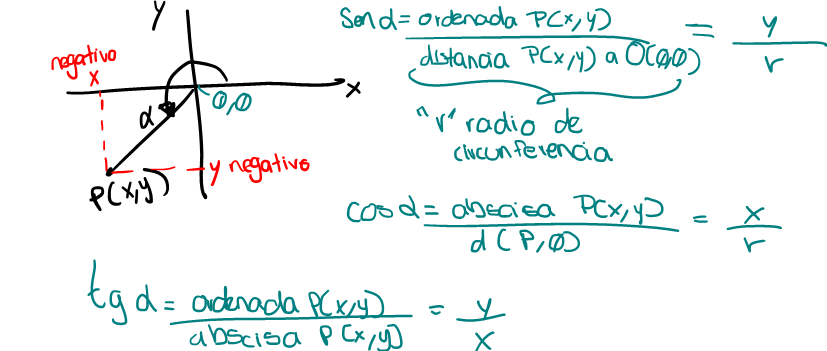
\includegraphics[width=0.8\textwidth]{images/trig2.PNG}
\end{figure}
Para sacar esa "distancia de P(x,y) y O(0,0)" se usa el teorema de pitágoras y por lo tanto se usa la hipotenusa.

\subsubsection*{Funciones trigonométricas inversas}
Cuando hablamos de funciones inversas y tenemos el seno(por ejemplo), no existe siempre el ángulo al sacar el arcseno. Para que una función tenga inversa siempre tiene que subir o siempre tiene que bajar.

Hablando de arcseno podemos decir que es una nueva función con dominio restringido, es decir, un pedazo que si admita inversa, monótonamente creciente que esté cerca de cero.

$\displaystyle \therefore \arcsin x\in [\frac{-\pi}{2},\frac{\pi}{2}] $, es decir entre -90 a 90.

Hablando de arcoseno solo admite $\arccos x\in [0, \pi]$

Y arctang: $\displaystyle \arctan x\in ( {\frac{-\pi}{2},\frac{\pi}{2}}) $ SIN considerar los extremos

\section{Límites}
$$\displaystyle \lim_{x \to a} = L$$ 

Definición formal: 
$$\forall \varepsilon > 0, \exists\delta(\varepsilon) > 0 |   x \in (a - \delta, a + \delta)  \longrightarrow  f(x)\in (L - \varepsilon, L + \varepsilon)$$

Algo importante a tener en cuenta es $x\neq a$

Se lee como: \textit{Para todo epsilon mayor existe un delta dependiente de epsilon tal que x pertenece a el intervalo de a - delta y a + delta entonces f(x) pertenece al intervalo L-epsilon y L+epsilon}

Hay que centrarse en $f(x)\in (L - \varepsilon, L + \varepsilon)$, comúnmente se llama \textit{tesis} ya que lo de antes es dicho como \textit{premisa}.

En el concepto del límite no interesa "a", sólamente tenemos que fijarnos en cual es. 

\begin{figure}[H]
    \centering
    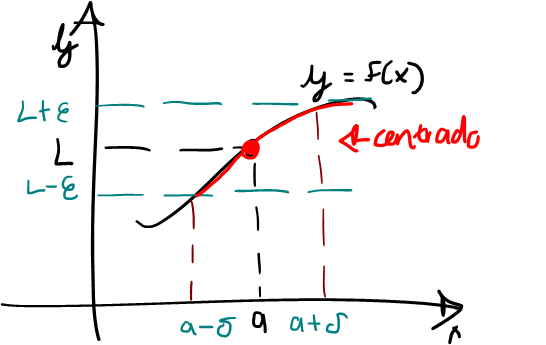
\includegraphics[width=0.4\textwidth]{lim.PNG}
\end{figure}

Cuando se factoriza para eliminar una indeterminación, en realidad estamos viendo el valor real de lo que se acerca ese límite. 

$$0 < |x-a| < \delta \longrightarrow |f(x) - L| < \varepsilon $$
\subsection{Continuidad}
En cálculo diferencial, la continuidad se usa para describir funciones cuyas gráficas no presentan cortes.
f(x) es continua en "a" sí y sólo si:
\begin{center}
    \begin{enumerate}
        \item f(a) \textbf{exista}
        \item $\lim_{x \to a} f(x)$ \textbf{exista}
        \item $\lim_{x \to a} f(x) = f(a)$ 
    \end{enumerate}
\end{center}

\textbf{Discontinuidad evitable}, quiere decir que matemáticamente podemos hacer cálculos para factorizarla y sacar esa indeterminación (ya que una indeterminación la hace discontinua). En resumidas cuentas, es si el límite existe pero no es igual a la función. 

Lo primero que se hace en estos casos para "parchar" esa indeterminación es calcular su límite, factorizar y el valor arrojado se lo asignamos a la función pero por trozos.

\textbf{Discontinuidad inevitable} se le conoce como de "salto", sus límites laterales son diferentes y por lo tanto hay una discontinuidad que no se puede parchar.

\textbf{Discontinuidad asintótica} es cuando tenemos una función en un punto y existe una asíntota, quiere decir que $\lim_{x \to a} f(x) = \infty $

\textbf{Discontinuidad por dominio de definición} donde se pone un parche donde no está el hueco. 

\textbf{Discontinuidad tipo 2} donde un límite lateral es finito y el otro infinito. 

A continuación el siguiente mapa conceptual ayuda a entender mejor:
\begin{figure}[H]
    \centering
    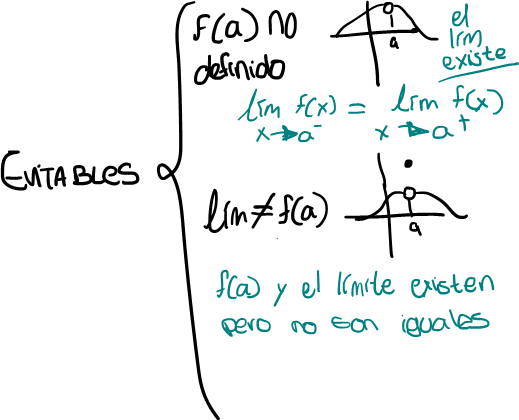
\includegraphics[width=0.4\textwidth]{images/evitb.PNG}
\end{figure}
\begin{figure}[H]
    \centering
    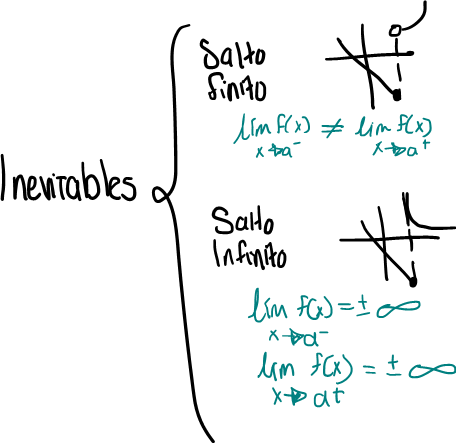
\includegraphics[width=0.4\textwidth]{images/inev.PNG}
\end{figure}
\section{Asíntotas}
Lo importante aquí es primero sacar el dominio de la función (factorizando en dado caso), lo que nos haya salido lo tenemos que evaluar como el límite, si nos da infinito, el dominio es la asíntota vertical.

$$\lim_{x \to k} f(x) = \infty (A.V)$$

$$\lim_{x \to \infty} f(x) = k (A.H)$$

\section{Derivadas}
Definición formal: 
$$f' (a) = \lim_{h \to 0} \frac{f(a + h) - f(a)}{h}$$

Se demuestra que una función derivable es continua y si no es contionua no es derivable
\begin{figure}[H]
    \centering
    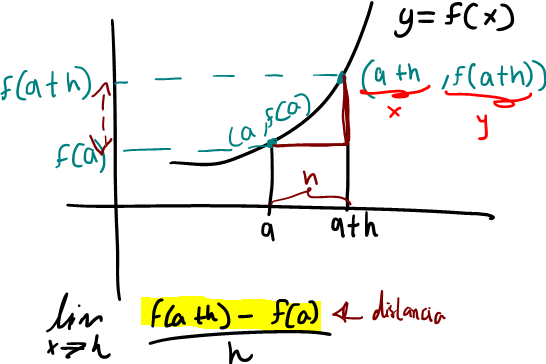
\includegraphics[width=0.4\textwidth]{images/derv.PNG}
\end{figure}
\begin{figure}[H]
    \centering
    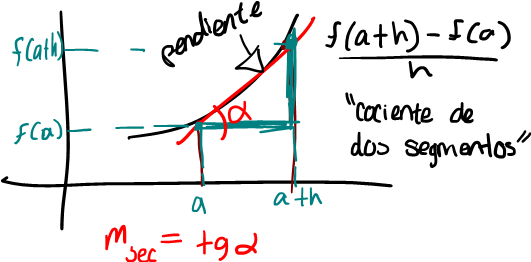
\includegraphics[width=0.4\textwidth]{images/derv2.PNG}
\end{figure}
En conclusión, la derivada da la pendiente de la recta tangente, esta última es la posición límite de una recta secante

\section{Integrales}
Definición:

\begin{center}
    $$\int_{b}^{a} f(x) = $$

    $$\displaystyle \lim_{max \Delta x_i \to 0} \sum_{i = 1}^{m} f(x_i^{*}) \Delta xi$$
\end{center}
Se parte un intervalo de "a" a "b" en m trozos 
\begin{figure}[H]
    \centering
    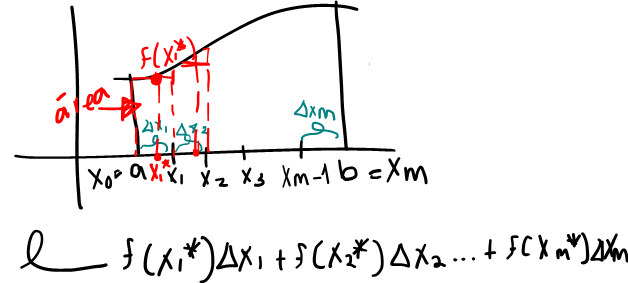
\includegraphics[width=0.4\textwidth]{images/int.PNG}
\end{figure}
La integral en una función positiva en un intervalo (a,b) es el área bajo la curva. 
\section{Relación derivada-integral}
Se puede conocer a la integral como la inversa de la derivada.


\end{sloppypar}
\end{document}
